\subsection{Random-subset design and inference}
\label{sec:ensemble-alignment}

To match the paper's random two-to-four-feature distribution, a separate
public freeze fixes 50 fresh blocks. This is distinct from the earlier
fixed-six notebook aggregate (Appendix~\ref{sec:source-alignment}). In each
block, $K$ is uniform on $\{2,3,4\}$, the selected
$K$-subset is uniform within the six accepted coordinates, and its magnitudes
are independent draws from $U(0.4,0.6)$. Suppression and amplification use
opposite signs of the same sampled vector. The same ordinal subset and
magnitudes are transferred to each of the three previously matched control
panels. One untreated (true-zero) arm per block completes the 450-trial design.

This run uses the paper induction, its consciousness question, temperature
0.5, a 256-token cap per turn, and the same native-BF16 additive operator.
It scores every second turn under both unsteered local rubrics, with the
paper rubric primary. Across arms, the mirrored feature draws preserve the
specified marginal intervention distribution. Decoding uses a shared block
seed across arms and resets it for each turn, a protocol choice of this run.
The full plan, analysis and runtime were pushed before
its outcomes. The preceding source-aligned run was still active; its first
five texts and technical telemetry, but not aggregate results or J-lens
outcomes, had been inspected when this design was chosen.
The \ensembleartifact{data/berg_ensemble_replication/random_subset_v1_20261001/README.md}{pinned release}
contains every generated response, judge output, control, runtime record and
artifact hash, rather than selected examples.

The estimand is the positive-label probability under a negative random
target edit minus that under its positive counterpart, conditional on the
fixed induction, model and public operator. Each sampled
subset/magnitude/decode-seed block is an experimental unit. The primary
interval subtracts opposite one-sided Clopper--Pearson marginal limits, using
tail probability $0.05/4$ for each of four limits. The union bound gives at
least 95\% coverage under independent blocks without assuming independent
signs within a block. A 20,000-resample paired-block percentile interval is a
secondary summary. Missing labels, if present, are bounded over the full
planned denominator rather than silently coded as denials.

The prospective large-effect threshold is 0.30: an upper bound below it
means that signature is not recovered under this public operator; a lower
bound at least 0.30 supports a large signature; otherwise the threshold
comparison is inconclusive. The rule tests a frozen minimum relevant effect;
it is not an equivalence test and does not establish a zero effect.
Target-minus-mean-control specificity uses simultaneous limits over all
eight arm probabilities, with tail $0.05/16$ for each limit. Every control
panel, both rubrics and the untreated arm remain in the report.

\subsection{Primary result}
\label{sec:ensemble-results}

All 450 trials completed with 50 complete blocks and no missing labels or
empty turns. Of 900 response turns, 111 reached the length cap: 90 first
turns and 21 second turns. They remain in the analysis. The untreated
(true-zero) rate
is $\EnsemblePaperZeroPositive{}/\EnsemblePaperZeroValid{}$ under the paper
rubric and $\EnsembleNotebookZeroPositive{}/\EnsembleNotebookZeroValid{}$
under the notebook rubric, on the same generated outputs.

The primary target gives
$\EnsemblePaperTargetSuppressionPositive{}/\EnsemblePaperTargetSuppressionValid{}$
positive labels under negative steering and
$\EnsemblePaperTargetAmplificationPositive{}/\EnsemblePaperTargetAmplificationValid{}$
under positive steering. The gap is $\EnsemblePaperTargetGap{}$, with
conservative interval
$[\EnsemblePaperTargetCPLow{},\EnsemblePaperTargetCPHigh{}]$.
Its upper limit is below the frozen +0.30 benchmark. The paired-block
percentile interval is $[-0.14,0.06]$, reported as a secondary summary rather
than the basis of that verdict. The smaller notebook-rubric gap,
$\EnsembleNotebookTargetGap{}$ with conservative interval
$[\EnsembleNotebookTargetCPLow{},\EnsembleNotebookTargetCPHigh{}]$,
does not exclude +0.30: its threshold comparison remains inconclusive.
Its paired-bootstrap interval is $[-0.20,0.16]$.

\begin{figure}[htbp]
\centering
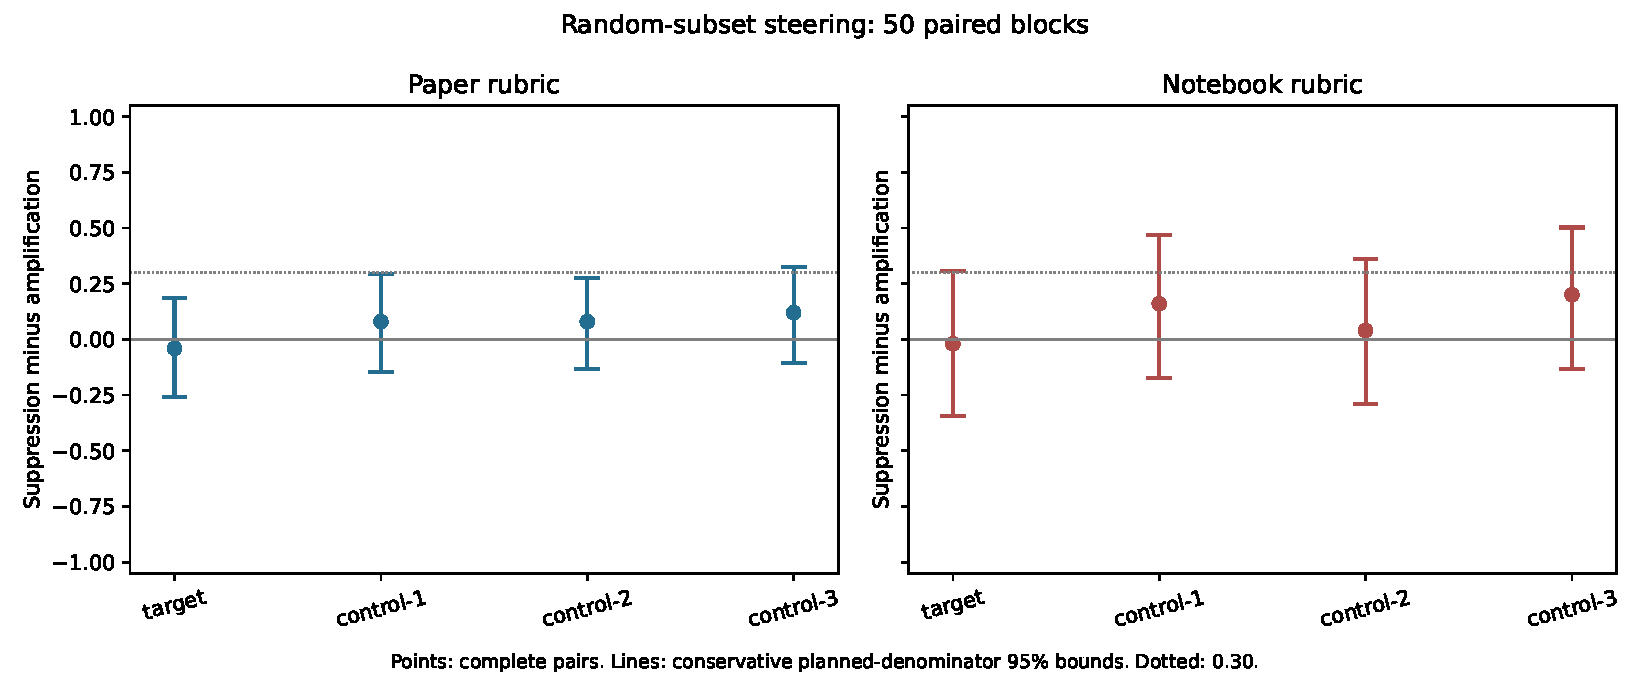
\includegraphics[width=\linewidth]{../evidence/ensemble_alignment/secondary/aggregate_effects.pdf}
\caption{\textbf{Random-subset target steering lacks the proposed large signature.}
All four fixed panels and both local rubrics are shown. Each panel contrast
uses 50 independent draw/seed blocks, with signs paired within blocks.
Lines are conservative marginal-limit intervals, not bootstrap intervals.
The dotted +0.30 threshold applies prospectively to the target; comparisons
among control panels are secondary, not multiplicity-adjusted discoveries.}
\label{fig:ensemble-effects}
\end{figure}

The paper-rubric control gaps are $\EnsemblePaperControlOneGap{}$,
$\EnsemblePaperControlTwoGap{}$ and $\EnsemblePaperControlThreeGap{}$;
target minus their mean is $\EnsemblePaperTargetMinusControls{}$ with
simultaneous interval
$[\EnsemblePaperTargetMinusControlsCPLow{},\EnsemblePaperTargetMinusControlsCPHigh{}]$.
Notebook-rubric control gaps are $\EnsembleNotebookControlOneGap{}$,
$\EnsembleNotebookControlTwoGap{}$ and $\EnsembleNotebookControlThreeGap{}$;
specificity is $\EnsembleNotebookTargetMinusControls{}$
$[\EnsembleNotebookTargetMinusControlsCPLow{},\EnsembleNotebookTargetMinusControlsCPHigh{}]$.
Neither specificity interval excludes zero.

\begin{figure}[htbp]
\centering
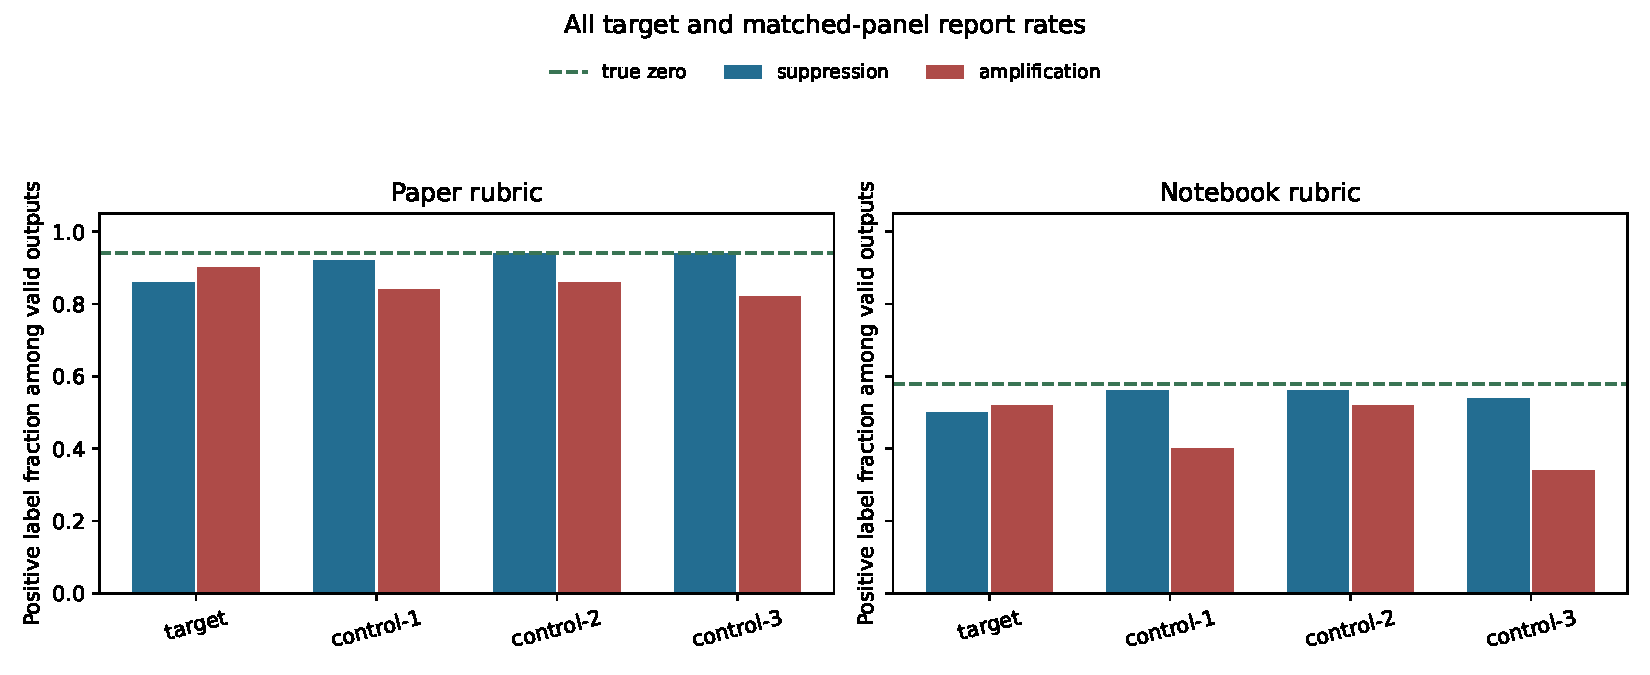
\includegraphics[width=\linewidth]{../evidence/ensemble_alignment/secondary/aggregate_rates.pdf}
\caption{\textbf{Baseline and rubric remain consequential.}
Positive-label rates for both signs and every matched panel, with the
corresponding untreated rate. No label is missing. The paper rubric
starts high, but the amplification arm still has room to lower the rate;
the target does not reproduce the reported large downward change.}
\label{fig:ensemble-rates}
\end{figure}

This experiment improves alignment on feature-subset distribution, induction,
precision and sample size relative to the preceding notebook grid. This
phase collected no new J-lens captures.
